%!TEX root = /Users/manunavjeevan/Desktop/Research/ML + Lasso/Annotated Literature Review/litNotesML.tex

\section{Generalized Random Forests; \textit{\small Susan Athey, Julie Tibshirani, Setfan Wager (AOS, 2018)}}
This paper can be found on ArXiv \href{https://arxiv.org/pdf/1610.01271.pdf}{here}.
\subsection{Introduction}
\begin{itemize}
	\item Random Forests first introduced by Breiman (2001)
	\item Used for conditional mean estimation. Given a data generating distribution for $(X_i, Y_i) \in \mathscr{X}\times\mathbb{R}$, want to estimate 
	\begin{equation}
		\mu(x) = \mathbb{E}[Y| X_i = x]
	\end{equation}
	\item Paper extends this to a flexible method for estimating any quantity $\theta(x)$ defined via local moment conditions. Specifically, given data $(X_i, O_i) \in \mathscr{X}\times\mathscr{O}$, we want forest based estimates of $\theta(x)$ defined by a local moment condition of the form 
	\begin{equation}\label{MC1}
		\mathbb{E}[\psi_{\theta(x), \nu(x)}(O_i)|X_i = x] = 0, \hbox{ }\text{ for all }x\in \mathscr{X}
	\end{equation}
	where $\psi(\cdot)$ is a score function and $\nu(\cdot)$ is an optional nuisance parameter.
	\begin{itemize}
		\item For example, if we model the distribution of $O_i$ conditional on $X_i$ to have a density $f_{\theta(x), \nu(x)}(\cdot)$ then the moment condition one with $\psi = \nabla \log f_{\theta(x), \nu(x)}(\cdot)$ ideintifies the local maximum likelihood 
		\item Substantive application involved heterogeneous treatment effect estimation with IV
	\end{itemize}
	\item Aim is to build a famly of non-parametric estimators that inherit desirable empirical properties of regression forests: stability, ease of use, flexible adaptation to different functional forms
	\item Regression forests typically understood as ensemble methods
	\begin{equation*}
		\hat{\mu}(x) = B^{-1} \sum_{b= 1}^B \hat{\mu}_b(x)
	\end{equation*}
	because individual trees have low bias but high variance, this averaging stabilizes predictions. 

	This method may not work as well when we are given moment conditions as in \ref{MC1}. Noisy solutions to moment equations are generally biased and averaging would do nothing to alleviate the bias.

	\item Cast forests as a type of adaptive locally weighted estimatior that first uses a forest to calculate a weighted set of neighbors for each test point $x$ and then solves a plug-in version of \ref{MC1} using these neighbors.
	\begin{itemize}
		\item Previously advocated by Hotheorn et. al (2004) in the context of survival analysis and by Meinshausen (2006) for quantile regression
		\item For conditonal mean estimation the averaging and weighting views of forests are equivalent, for moment conditions the weighting based perspective proves more effective
	\end{itemize}
	\item Bulk of this paper is devoted to theoretical analysis of generalized random forests
\end{itemize}
\subsubsection{Related Work}
\begin{itemize}
	\item Idea of local maximum likelihood has a long history. Core idea: when estimating parameters at a particular value of covariates, a kernel weighting function is used to place more weight on nearby observations in the covariate space. Paper replaces the kernel weighting function with forest based weights. 
	\begin{itemize}
		\item Weights dervied from the fraction of trees in which an observation appears in the same leag as the target value of the covariate vector.
		\item If the covariate space has more than a few dimensions kernel methods can suffer from curse of dimensionality.
	\end{itemize}
\end{itemize}
\subsection{Generalized Random Forests}
\begin{itemize}
	\item In the standard classification or regresion forests proposed by Breiman (2001), prediction for a particular point $x$ is determined by averaging predictions across an ensemble of different trees.
\end{itemize}
Suppose that we have $n$ independent and identically distributed samples, indeced $i = 1, \dots, n$. For each sample, access to an observable quantity $O_i$ that encodes information relevant to estimation $\theta(\cdot)$, along with a set of auxilary covariates $X_i$.
\begin{itemize}
	\item In the case of NPR; $O_i = \{Y_i\}, Y_i \in \mathbb{R}$, though in general it may contain richer information. 
	\begin{itemize}
		\item In the case of treatment effect estimation weith exogeneous treatment assignment, $O_i = \{Y_i, W_i\}$ where $W_i$ represents the treatment assignment.
	\end{itemize}
\end{itemize}
Given this type of data, the goal is to estimation solutions to local estimation equations of the form $\mathbb{E}[\psi_{\theta(x), \nu{x}}(O_i)|X_i = x] = 0$ (Eq. \ref{MC1}), for all $x \in \mathscr{X}$. We care about $\theta(x)$ and $\nu(x)$ is a nuisance parameter. 

One approach: Define some similarity weights $\alpha_i(x)$ that measure the relevance of the $i$-th training example to fitting $\theta(\cdot)$ at $x$ and then fit the target of interest via an empirical version of the estimation equation 
\begin{equation}\label{eq:mc_sample}
	\left(\hat{\theta}(x), \hat{\nu}(x)\right) \in \arg\min_{\theta,\nu}\left\{\left\Vert \sum_{i=1}^n \alpha_i(x)\psi_{\theta,\nu}(O_i)\right\Vert_2\right\}
\end{equation}
If the expresion has a unique root we can say that the estimators ``solve'' eq. \ref{eq:mc_sample}. Weights used in the above equations are traditionally obtained via a deterministic kernel function, perhaps with an adaptively chosen bandwith parameter. This method of choosing weights suffers from curse of dimensionality. This paper uses forest-based algorithms to adaptively learn better, problem specifc, weights, $\alpha_i(x))$ that van be used in conjunction with eq. \ref{eq:mc_sample}.
\begin{enumerate}
	\item Grow a set of $B$ trees indicated by $b=1, \dots, B$ and, for each such tree, define $L_b(x)$ as the set of training examples falling in the same ``leaf'' as $x$.
	\item Define the weights as the frequency with with the $i$-th training example falls into the same leaf as $x$:
	\begin{equation}\label{eq:alpha_bi}
		\alpha_{bi}(x) = \frac{\mathbf{1}\{X_i \in L_b(x)\}}{|L_b(x)|}
	\end{equation}
	These weights sum to 1 and define the forest based adaptive neighborhood of $x$.
\end{enumerate}
Construction of the trees and the ``neighbor'' sets $L_b(x)$ require some subtleties. In particular, construction will rely on both subsampling and specific form of sample splitting to achieve consistency.
\begin{itemize}
	\item For the special case of regression trees, the weighting based definition of a random forest is equivalent to the standard ``average of trees'' perspective taken in Breiman (2001) 
\end{itemize}

\subsubsection{Splitting to Maximize Heterogeneity}
Seek trees that, when combined into a forest, induce weights $\alpha_i(x)$ that lead to good estimates of $\theta(x)$. Random forests use recursive partitioning on subsamples to generate these weights $\alpha _i(x)$. Algorithm considered in the paper mimics Breiman (2001) as closely as possible, while tailoring splitting to focus on heterogeneity in $\theta(x)$. 

Use a greedy algorithm to look for splits. Each split starts with a parent node $P \subset \mathscr{X}$. Given a sample $\mathscr{J}$, define $(\hat{\theta}_P, \hat{\nu}_p)(\mathscr{J})$ as 
\begin{equation}\label{eq:theta_nu_sample}
\left(\hat{\theta}_P,\hat{\nu}_P \right) \in \arg\min_{\theta,\nu}\left\{\left\Vert \sum_{\{i \in \mathscr{J}, X_i \in P\}} \psi_{\theta,\nu}(O_i)\right\Vert_2\right\}\footnote{Minimize the $L_2$ norm because we want the moment condition to be as close to zero as possible}
\end{equation}
This contrasts to (\ref{eq:alpha_bi}) because there is no weighting. Would like to divide $P$ into two children, $C_1, C_2 \subset \mathscr{X}$ using an axis-aligned cut\footnote{Axis-aligned means that the cut considers only one variable at a time. See \href{https://www.researchgate.net/figure/A-decision-boundary-generated-by-a-an-axis-aligned-and-b-an-oblique-split-function_fig1_290508933}{link} for a visual representation} to improve the accuracy of our $\theta$ estimates as much as possible. Formally, this means seeking to minimize 
\[\err(C_1,C_2) = \sum_{j = 1,2} \mathbb{P}\left[X\in C_j|X\in P\right]\mathbb{E}\left[\left(\hat{\theta}_{C_j} - \theta(X)\right)^2 | X\in C_j\right]\]
where $\hat{\theta}_{C_j}(\mathscr{J})$ are fit over children $C_j$ as in eq. \ref{eq:theta_nu_sample}. Expectations are taken over both the randomness in $\hat{\theta}_{C_j}(\mathscr{J})$ and a new test point $X$. This is to say, the $\err$ function is the ``true'' function we want to minimize. 

Many standard regression tree implementations choose splits by minimizing prediction error of the node. This corresponds to $\err(C_1,C_2)$ with plug in estimators from the training sample. Athey and Imbens (2016) study sample-splitting trees to estimate a treatment effect. They propose an unbiased, model-free (nonparametric) estimate of $\err(C_1, C_2)$ using an overfitting penalty as in Mallows (1973). In the general moment condition setting as defined by \ref{MC1} this may not work. If $\theta(x)$ is defined only by a moment condition, then we do not in general have access to an unbiased, model free estimate of the criterion $\err(C_1,C_2)$. The following proposition tries to address this.

\begin{prop}
\label{prop1}
	Suppose that the basic assumption detaled later in Section 3 hold, and that the parent node $P$ has a radius smaller than $r >0$. We write $n_P = |\{i \in \mathscr{J}: X_i \in P\}|$ for the number of observations in the parent and $n_{C_j}$ for the number of observations in each child and define 
	\begin{equation}
	\label{eq:delta_criterion}
		\Delta(C_1,C_2) := n_{C_1}n_{C_2}\big/n^2_P\left(\hat{\theta}_{C_1}(\mathscr{J}) - \hat{\theta}_{C_2}(\mathscr{J})\right)^2
	\end{equation}
	where $\hat{\theta}_{C_1}, \hat{\theta_{C_2}}$ are the solutions to the estimating equation computer in the children, following eq. \ref{eq:theta_nu_sample}. Then, treating the child notes $C_1,C_2$ as well as the corresponding counts $n_{C_1}, n_{C_2}$ as fized, and assuming that $n_{C_i} \gg r^{-2}$ we have that 
	\[\err(C_1,C_2) = K(P) - \mathbb{E}[\Delta(C_1,C_2)] + o(r^2)\]
	where $K(P)$ is a deterministic term that measures the purity of the parent node that does not depend on how the parent is split, and the $o$-term incorporates terms that depend on sampling variance. 
\end{prop}

Motivated by this observation, paper considers splits that make the above $\Delta$-criterion in eq. \ref{eq:delta_criterion} large.

\subsubsection{The Gradient Tree Algorithm}

Above discussion provides conceptual guidance on how to pick good splits. But actually optimizing the criterion $\Delta(C_1,C_2)$ over all possible axis-aligned cuts while also solving for $(\hat{\theta}, \hat{\nu})$ at each leaf can be computationally expensive. To avoid the issue, paper proposes optimizing an approximate criterion $\tilde{\Delta}(C_1,C_2)$ using gradient based approximations for $(\thetaH_{C_1},\thetaH_{C_2})$. For each child $C$, use $\thetaT_C \approx \thetaH_C$ as follows: First, compute $A_P$ as any consistent estimate for the gradient of the expectation of $\psi$ function; i.e, $A_P \rightarrow \nabla\mathbb{E}[\psi_{\thetaH_P,\nuH_P}(O_i)]$. Then, set 
\begin{equation}
	\label{eq:thetaT_def}
	\thetaT = \thetaH - \frac{1}{|\{i: X_i \in C\}|} \sum_{\{i: X_i \in C\}} \xi^T A_P^{-1} \psi_{\thetaH_P, \nuH_P}(O_i)
\end{equation}
$\thetaH_P$ and $\nuH_P$ are obtained by solving eq. \ref{eq:theta_nu_sample} once in the parent node and $\xi$ is a vector that picks out the $\theta$ coordinate from the vector $(\theta, \nu)$. When $\psi$ is itself continuously differentiable we use 
\begin{equation}
	\label{eq:Ap_def}
	A_P = \frac{1}{|\{i: X_i \in P\}|} \sum_{\{i: X_i \in P\}} \nabla \psi_{\thetaH, \nuH}(O_i)
\end{equation}
Algorithim's recursive partitioning scheme reduces to alternatively applying the following two steps. First, in a \textbf{labeling step}, compute $\thetaH_P, \nuH_P$ and the derivative matrix $A_{P}^{-1}$ on the parent data as in eq. \ref{eq:theta_nu_sample}, and use them to get the psuedo-outcomes 
\begin{equation}
	\label{eq:labeling_step}
	\rho_i = -\xi^T A_P^{-1} \psi_{\thetaH_P, \nuH_P}(O_i) \in \mathbb{R}
\end{equation}
Next in a \textbf{regression step}, run a standard CART regression split on the outcome $\rho_i$. Specifically, we split $P$ into two axis-aligned children $C_1$ and $C_2$ such as to maximize the criterion 
\begin{equation}
	\label{eq:regression_step_criterion}
	\DeltaT(C_1,C_2) = \sum_{j=1}^2 \frac{1}{|\{i: X_i \in C_j\}|}\left(\sum_{\{i:X_i \in C_j\}}  \rho_i\right)^2
\end{equation}
Once the regression step has been executed, relabel observations in each child by solving the estimating equation, and continue on recursively. \footnote{This whole section is really going over the recursive step of the algorithm}
\begin{itemize}
	\item In the simplest case of least square regression (mean regression), with $\psi_{\theta(x)}(Y) = Y - \theta(x)$ the labeling step in eq. \ref{eq:labeling_step} doesn't change anything. The second step in maximizing eq. \ref{eq:regression_step_criterion} corresponds to the usual way of making splite in Breiman (2001).
	\begin{itemize}
		\item Special structure of the problem considered in this paper is encoded into eq. \ref{eq:labeling_step}.
	\end{itemize}
\end{itemize}
This approach is expected to provide more consistent computational performance than optimizing \ref{eq:delta_criterion} at each step. Computation in growing a tree is typicall dominated by the split-selection step, so it is critical for this step to be implemented as effeciently as possible. Conversely the labeling step is only solved once per node, so is less performance sensitive. The algorithms for doing this are specified below:

\begin{figure}[htbp]
	\centering
	\subfigure[Algorithm 1]{%
	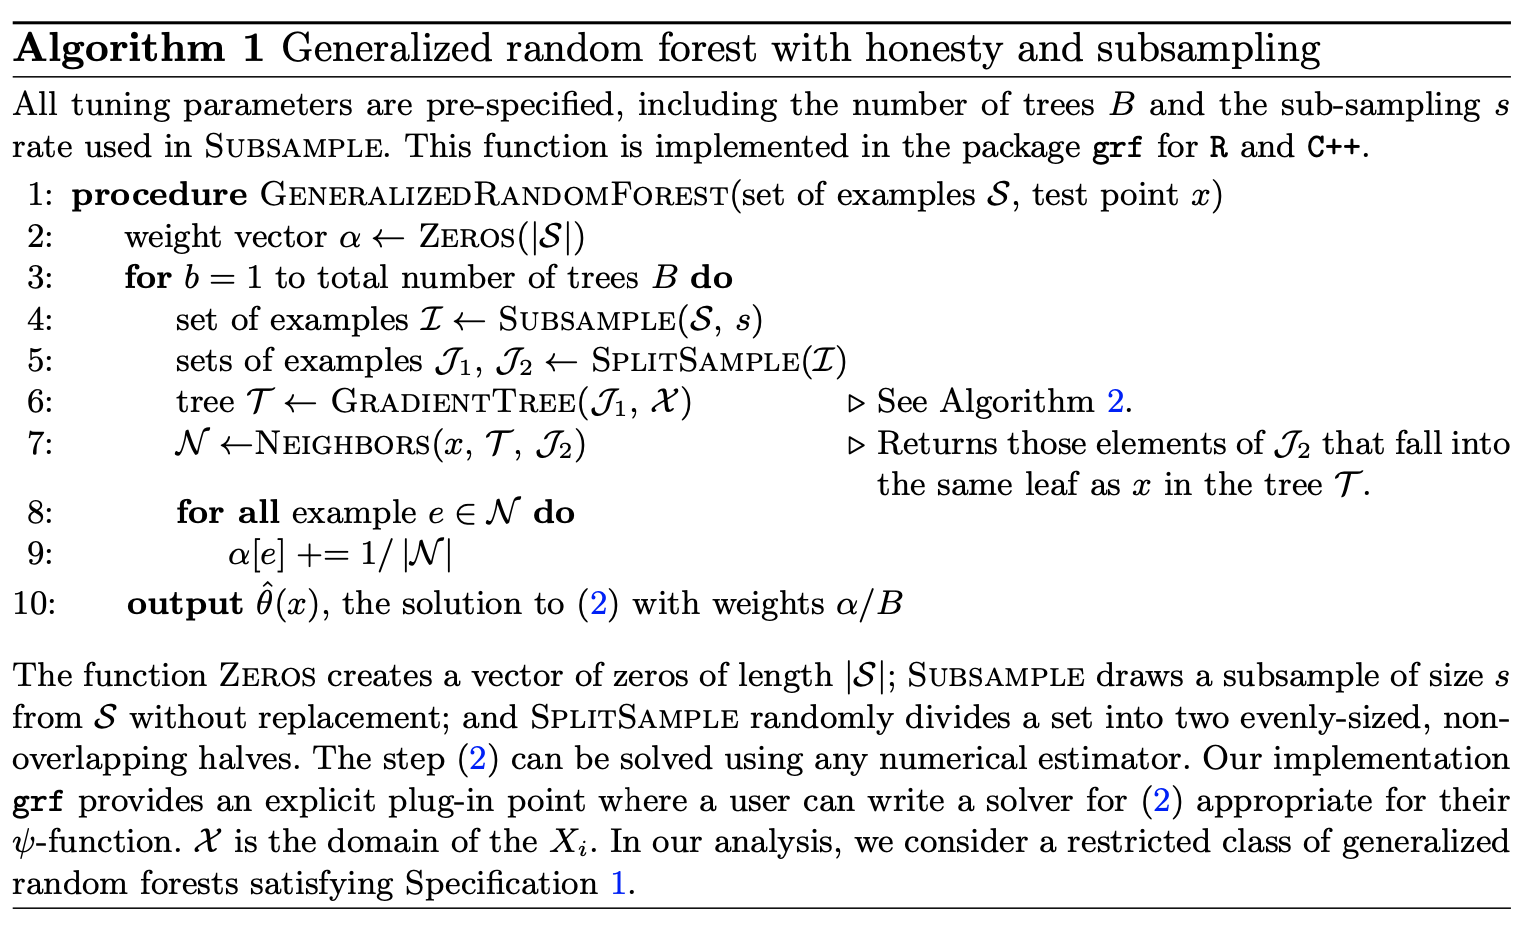
\includegraphics[width = 0.475\textwidth, height = 4.5cm]{Figures/grf/grfAlgo1.png}
	}
	\subfigure[Algorithm 2]{%
	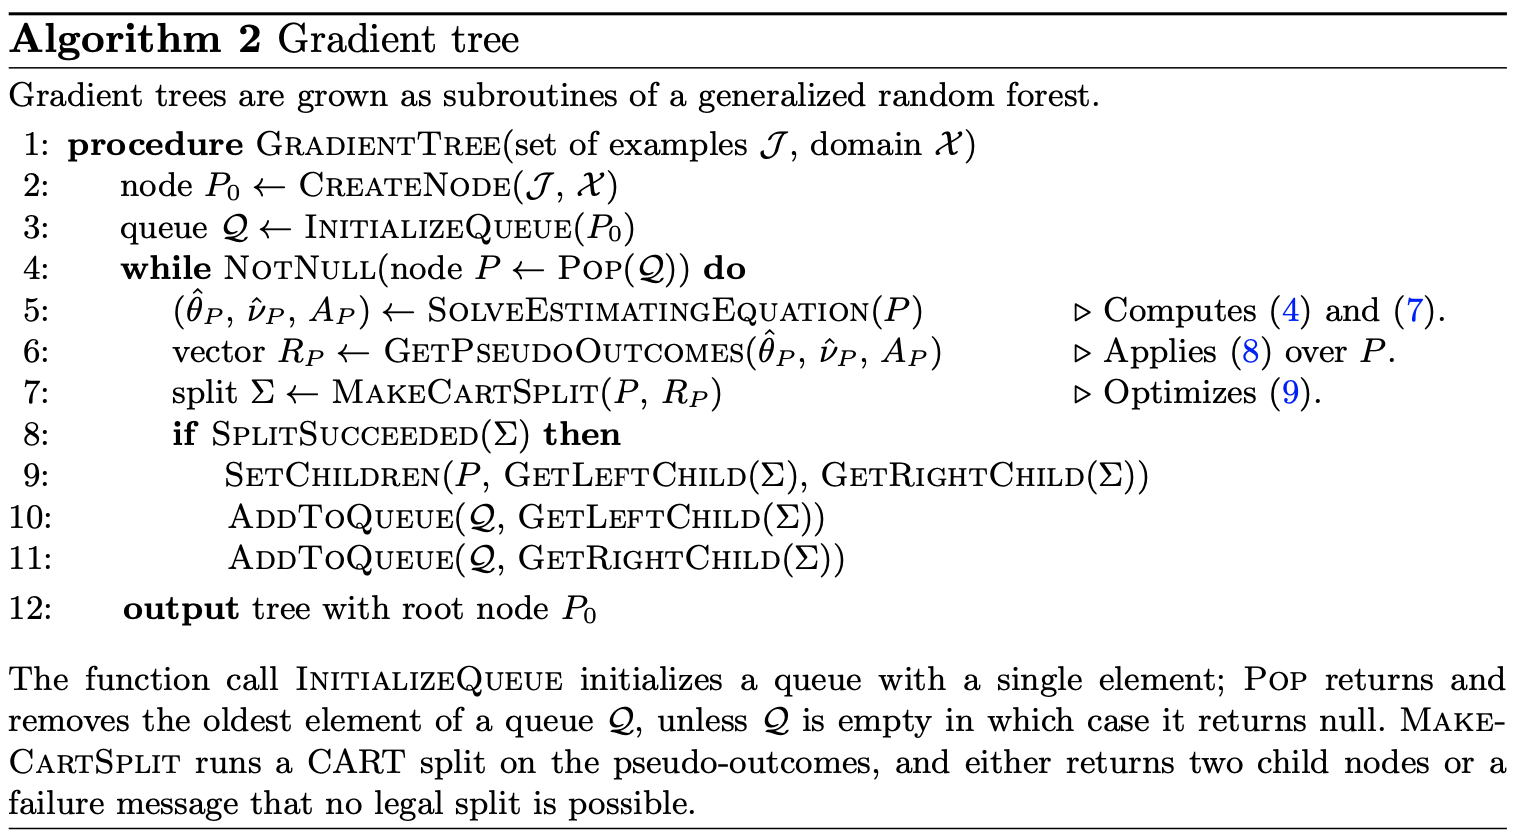
\includegraphics[width = 0.475\textwidth, height = 4.5cm]{Figures/grf/grfAlgo2.png}
	}
	\caption{Algorithms for growing generalized random forests}
\end{figure}

In contrast to using a regression splitting criterion as in \ref{eq:regression_step_criterion}, which only requres a single pass over the data in the parent node, directly optimizing the original criterion in eq. \ref{eq:delta_criterion} may require optimizing at every possible candidate split. This sort of gradient based approximation also underlies other popular statistical algorithms, including gradient boosting (Friedman, 2001) and model based recursive partitioning algorithm of Zeileis, Hothorn, and Hornik (2008).

Paper can verify that the error from using the approcimate criterion $\DeltaT$ instead of the exact $\Delta$-criterion is within the tolerance used to motivate the $\Delta$-criterion in Proposition $1$, thus suggesting that use of it may not result in too much ineffeciency. Consistent estimates of $A_P$ can, in general, be derived directly, without relying on the proposition below
\begin{prop}
Under the conditions of Proposition \ref{prop1}, if $|A_P - \nabla\mathbb{E}[\psi_{\thetaH_P, \nuH_P}(O_i)|X_i \in P]| \rightarrow_P 0$, then $\Delta(C_1, C_2)$ and $\DeltaT(C_1,C_2)$ are approximately equivalent in that 
\[\DeltaT(C_1,C_2) = \Delta(C_1,C_2) + o_P\left(\max\{r^2, 1/n_{C_1}, 1/n_{C_2}\}\right)\]
\end{prop}

Now, given a practical splitting scheme for growing individual trees, we want to grow a forest that allows for consistent estimation of $\theta(x)$ using \ref{eq:theta_nu_sample} using the forest weights in eq. \ref{eq:alpha_bi}. Each tree will provide small, relevant neighborhoods for $x$ that will lead to noisy estimates of $\theta(x)$; then we may hope that forest based aggregation will provide a single larger but still relevant neighborhood of $x$ that yields stable estimates $\thetaH(x)$. Rely on two conceptual ideas that have proven to be succesful in the literature on forest-based least-squares regression. 
Training trees on subsamples of the data nd a subsampling splitting technique called ``honesty''.

\subsection{Asymptotic Analysis}

Aim of this section is to establish asymptotic Gaussianity of the $\thetaH(x)$ and of providing tools for statistical inference about $\theta(x)$. The covariate space and the parameter space are both subsets of Euclidean space. Specifically $\mathscr{X} = [0,1]^p$ and $(\theta, \nu) \in \mathscr{B} \subset \mathbb{R}^k$ for some $p,k > 0$ and $\mathscr{B}$ is a compact subset.\footnote{This seems to restrict $\theta$ to be semiparametric. I don't think that is the right interpretation though. $\theta(x)$ can still be an arbitrary function taking values on a the real line.} Moreover, we assume that $X$ has a density that is bounded away from 0 and from above. This is a weaker requirement in the forest prediction space since trees and forests are invariant to monotone rescaling of the features.

Some practically interesting cases, such as quantile regression involve discontinuous score functions $\psi$, which complicates analysis. Here we assume that the spected score function
\begin{equation}
	\label{eq:expected_score}
	M_{\theta,\nu}(x) := \mathbb{E}[\psi_{\theta,\nu}(O)|X = x]
\end{equation}
varies smoothly in the parameters, even though $\psi$ itself may be discontinuous. For example, with quantile regression $\psi_{\theta}(Y) = \mathbf{1}(\{Y > \theta\}) - (1-q)$ is discontinuous in $q$ and $Y$, but $M_\theta(x) = \mathbb{P}[Y > \theta | X = x] - (1-q)$ is smooth whenever $Y|X=x$ has a smooth density. We add the following assumptions

\begin{assumption}{(Lipschitz $x$-signal) }
\label{as:lipschitz}
For fixed valued of $(\theta, \nu)$ we assume that $M_{\theta,\nu}(x)$ is Lipschitz continuous in $x$. 
\end{assumption}

\begin{assumption}{(Smooth identification) }
\label{as:smooth_id}
When $x$ is fixed, assume that the $M$-function is twice continuously differentiable in $(\theta, \nu)$ with a uniformly bounded second derivative, and that $V(x) := V_{\theta(x), \nu(x)}(x)$ is invertible for $x \in \mathscr{X}$, with $V_{\theta,\nu}(x) := \frac{\partial}{\partial(\theta, \nu)} M_{\theta,\nu}(x)\bigg|_{\theta(x),\nu(x)}$.
\end{assumption}
\begin{assumption}{(Lipschitz $(\theta, \nu)$-variogram) }
\label{as:lipschitz_variogram}
The score functions $\psi_{\theta,\nu}(O_i)$ have a continuous covariance structure. Writing $\gamma$ for the worst-case variogram and $\Vert \cdot \Vert_{F}$ for the Frobenius norm, then for some $L > 0$
\begin{align*}
\gamma\left( \begin{pmatrix} \theta \\ \nu \end{pmatrix}, \begin{pmatrix} \theta' \\ \nu' \end{pmatrix}    \right) &\leq L \left\Vert \begin{pmatrix} \theta \\ \nu \end{pmatrix} - \begin{pmatrix} \theta' \\ \nu' \end{pmatrix}  \right\Vert_2 \\
\gamma\left( \begin{pmatrix} \theta \\ \nu \end{pmatrix}, \begin{pmatrix} \theta' \\ \nu' \end{pmatrix}    \right) &:= \sup_{ x \in \mathscr{X} }\{\Vert \Var [\psi_{\theta, \nu}(O_i) - \psi_{\theta', \nu'}(O_i) | X_i = x]\Vert_F  \}
\end{align*}
\end{assumption}

\begin{assumption}{(Regularity of $\psi$) }
\label{as:psi_regularity}
The $\psi$-fucntions can be written as $\psi_{\theta, \nu}(O) = \lambda(\theta, \nu; O_i) + \zeta_{\theta, \nu}(g(O_i))$ such that $\lambda$ is Lipschitz-continuous in $\theta, \nu$ and $g: {O_i} \rightarrow \mathbb{R}$ is a univariate summary of $O_i$, and $\zeta_{\theta, \nu}: \mathbb{R} \rightarrow \mathbb{R}$ is any family of monotone and bounded functions
\end{assumption}
\begin{assumption}{(Existence of solutions) }
\label{as:existence}
We assume that, for any weights $\alpha_i$ with $\sum \alpha_i = 1$, the estimating equation returns a minimizer $(\thetaH, \nuH)$ that at least approximately solves the estimating equation: $\Vert \sum_{i=1}^n \alpha_i \psi_{\thetaH, \nuH}(O_i)\Vert_2 \leq C \max\{\alpha_i\}$ for some constant $C\geq 0$. 
\end{assumption}

\begin{assumption}{(Convexity) }
\label{as:convexity}
The score function $\psi_{\theta, \nu}(O_i)$ is a negative sub-gradient of a convex function, and the expected score $M_{\theta, \nu}(X_i)$ is the negative gradient of a strongly function. 
\end{assumption}
Assumption 3 holds trivially if $\psi$ is Lipschitz in the parameters. Assumption 4 is used to show that a certain empirical process is Donsker. The first 5 assumptions deal with local properties of the estimating equation and can be used to control the behavior of $(\thetaH(x), \nuH(x))$ in neighborhoods of the population parameter value $(\theta(x), \nu(x))$. The 6th assumption garuntees consistency. 

Consistency and Gaussianity results require using some specific settings for the trees from Algorithm 1. In particular, require that all trees are honest and regular in the sense of Wager and Athey (2018), as follows. In order to satisfy the minimum split probability condition below, our implementation relies on the device of Denil, Matheson and De Freitas (2014), whereby the number splitting variables considered at each step of the algorithm is random. Specifically, try $\min\{\max\{\Poisson(m), 1\},p\}$ variables at each step, where $m > 0$ is a tuning parameter.
\begin{specification}
All trees are symmetric in that their output is invariant to permuting the indices of training examples; make balanced splits in the sense that every split puts at least a fraction $\omega$ of the observations in the parent node into each child, for some $\omega > 0$; and are randomized in such a way that, at every split, the probability that the tree splits on the $j$-th feature. is bounded from below by $\pi > 0$. The forest is honest and built with subsample size satisfying $s/n \rightarrow 0$ and $s \rightarrow \infty$.
\end{specification}

These assumptions hold trivially under some weak assumptions for least squares and quantile regression.

\subsubsection{A Central Limit Theorem for Generalized Random Forests}

Now ready for asymptotic results. Note that regression forests are averages of regression trees grown over sub-samples and were thus be analyzed as $U$-statistics (Hoeffding, 1948). Unlike regression forest predictions, however, the parameter estimates $\thetaH(x)$ from generalized random forests are not averages of estimates made by different trees. Instead, we obtain $\thetaH$ by solving a single weighted moment equation as in eq. \ref{eq:mc_sample}. So existing proof strategies do not apply in thi setting. 

Tackle this problem using method of influence functions as described by Hampel (1974). In particular, we are motivated by the analysis of Newey (1994a). Core idea is to derive a sharp, linearized approzimation to the local estimatior, and then to analyze the linear approximation instead. Let $\ris(x)$ denote the influence function on the $i$-th observation with respect to the true parameter value, $\theta(x)$
\[\ris(x) := -\xi^TV(x)^{-1}\psi_{\theta(x),\nu(x)}(O_i)\]
Then, given any set of forest weights $\alpha_i(x)$ used to define the generalized random forest estimate $\thetaH(x)$ by solving (\ref{eq:mc_sample}) define a pseudo-forest 
\begin{equation}
\label{eq:thetaHat_appx}
	\thetaT^*(x) := \theta(x) + \sum_{i=1}^n \alpha_i(x) \ris(x)
\end{equation}
used to approximate $\thetaH(x)$. $\thetaT^*(x)$ is the output of an infeasible regression forest with weights $\alpha_i(x)$ and outcomes $\theta(x) + \ris(x)$. The upshot is that this is a $U$-statistic, which we know how to analyze. Because $\thetaT^*(x)$ is a linear function of the pseudo outcomes $\ris(x)$, it can be written as an average of pseudo-tree predictions $\thetaT^*(x) = \frac{1}{B}\sum_{b=1}^B \thetaT_{b^*}(x)$ where $\thetaT_{b^*}(x) = \sum_{i=1}^n \alpha_{ib}(x)(\theta(x)+ \ris(x))$. Then, because each individual pseudo-tree prediction $\thetaT_{b^*}$ is trained on a size $s$ usbsample of the training data, drawn without replacement, $\thetaT^*(x)$ is an infinite order $U$-statistic whose order corresponds to the subsample size. 
\begin{itemize}
	\item Arguments of Mentch and Hooker (2016) and Wager and Athey (2018) can be used to study the averaged estimator $\thetaT^*(x)$ using results on U-statistics from Hoeffding (1948) and Efron and Stein (1981)\footnote{The definition of U-statistic from Hoeffding (1948), via Wikipedia. Let $f: \mathbb{R}^r \rightarrow \mathbb{R}$ be a real-valued or complex-valued function of $r$ variables. For each $n\geq r$, the associated $U$-statistic $f_n:\mathbb{R}^n \rightarrow \mathbb{R}$ is equal to the average over ordered samples $\varphi(1), \dots, \varphi(r)$ or size $r$ of the sample values $f(x_\varphi)$. In otherwords $f_n(x_1, \dots, x_n) = \text{ave} f(x_{\varphi(1), \dots, x_\varphi(r)})$. By neccesity, each U-statistic is a symmetric function.} 
\end{itemize}
Difficulty in this proof stratefy is showing that $\thetaT^*(x)$ is a good approximation for $\thetaT(x)$. Following theorem establishes this. This is the only point where $\phi$ being the negative gradient of a convex loss function is used. 
\begin{theorem}
	\label{thm:consistency}
	Under Assumptions 1-6, estumatees $\thetaH(x), \nuH(x)$ converge in probability to $\theta(x), \nu(x)$.
\end{theorem}
Seperating the analysis of moment estimators into a local approcumation argument that hinges on consistency and a seperate result that estabilishes consistency is standard; see chapter 5.3 of Van Der Vaart (2000)\footnote{Textbook is \textit{Asymptotic Statistics} and it can be found in the google drive}

The remainder of analysis assumes that trees are grown on subsamples of size $s$ scalig as $s = n^\beta$ for some $\beta_{\min} < \beta < 1$ with 
\begin{equation}
	\label{eq:betaMin}
	\beta_{\min} := 1 - \left(1 + \pi^{-1}\left(\log(\omega^{-1})\right)\right)^{-1}
\end{equation}
where $\pi$ and $\omega$ are as in Specification 1. Scaling garuntees errors of forests are varaicne-dominated. 

\begin{lemma}
\label{thm:main-result}
Given Assumptions 1-5 and a forest trained according to Specification 1 with condition \ref{eq:betaMin} holding, suppose that the generalized random forest estimator $\thetaH$ is consistent for $\theta(x)$. Then $\thetaH(x)$ and $\thetaT^*(x)$ are coupled at the following rate
\begin{equation}
	\sqrt{\frac{n}{s}}\left(\theta^*(x) - \thetaH(x)\right) = \mathscr{O}_P \left( \max\left\{ 
	s^{-\frac{\pi \log \left( (1-\omega)^{-1}\right)}{2 \log \left( \omega^{-1}\right)}}, \left(\frac{s}{n}\right)^{\frac{1}{6}}\right\} \right)
\end{equation}
where $s$, $\omega$ and $\pi$ are as in Specification 1.
\end{lemma}
Given this coupling result, it now remains to study the asymptotics of $\thetaT^*(x)$. In doing so, important to know that $\thetaT^*(x)$ is exactly the output of an infeasible regression forest trained on outcomes $\theta(x) + \ris(x)$. So can apply results of Wager and Athey (2018) to this object. With this approach, authors show that, given \ref{eq:betaMin}m $\thetaT^*(x)$ and $\thetaH(x)$ are both asymptotically normal. Extending the argument can also so this for nuisance parameters, but noting that since tree is not trained to optimize nuisance, may not work well in finite samples. 
\begin{theorem}
	\label{thm:clt}
	Suppose Assumptions 1-6 hold and a forest is trained according to Specification 1 with trees grown on subsamples of size $s = n^\beta$ satisfying \ref{eq:betaMin}. Finally, suppose that $\Var[\ris(x)|X=x] > 0.$ Then, there is a sequence $\sigma_n(x)$ for which $(\thetaH_n(x) - \theta(x))/\sigma_n(x) \rightarrow \mathscr{N}(0,1)$ and $\sigma_n^2(x) = \polylog(n/s)^{-1}s/n$, where $\polylog(n/s)$ is a function that is bounded away from 0 and increases at most polynomially with the log-inverse sampling ratio $\log(n/s)$. 
\end{theorem}
\subsection{Confidence Intervals via the Delta Method}
Theorem \ref{thm:clt} can be used for statistical inference about $\theta(x)$. Given a consistent estimator $\hat{\sigma}_n(x)$ for $\sigma_n(x)$, Theorem \ref{thm:clt} can be paired with Sltutsky's lemma to verify
\[\lim_{n\rightarrow\infty} \mathbb{P}\left[\theta(x) \in \left(\thetaH(x) \pm \Psi^{-1}(1-\alpha/2)\hat{\sigma}_n(x)\right)\right] = \alpha\]
So to build asymptotically valid pointwise confidence intervales, it suffices to derive an estimator for $\sigma_n(x)$. Doing so requires leveraging coupling with the approximate pseudo-forest $\thetaT^*(x)$. Moreover, from the definition of $\thetaT^*(x)$, we directly see that 
\begin{equation}
	\label{eq:varThetaT*}
	\Var\left[\thetaT^*(x)\right] = \xi^T V(x)^{-1} H_n\left(x; \theta(x), \nu(x)\right)\left(V(x)^{-1}\right)^T \xi
\end{equation}
where $H_n(x;\theta, \nu) = \Var[\sum_{i=1}^n \alpha_i(x) \psi_{\theta,\nu}(O_i)]$. Authors then propose building confidence intervals via
\begin{equation}
	\label{eq:sigmaHat}
	\hat{\sigma}_n^2 := \xi^T \hat{V}_n(x)^{-1} \hat{H}_n(x) (\hat{V}_n(x)^{-1})^T \xi
\end{equation}
Coming up with consistent estimators of $V(x)$ is well studied and not so complex, according to the authors. Estimating $H$, however, can be difficult since it depends on the true forest score $\Psi(\theta(x), \nu(x)) = \sum_{i=1}^n \alpha_i(x) \psi_{\theta(x), \nu(x)}(O_i)$. To estimate this, they use a variant of the bootstrap of little bags algorithm (noisy bootstrap) proposed by Sexton and Laake (2009). They obtain the first consitency garuntees for this method for any type of forest, including regression forests. Notes about this are breifly given below

\subsubsection{Consistency of the Bootstrap of Little Bags}


